\section{多相机内外参联合标定}
\label{sec:camera_calib}

为了建立三维物体与二维照片之间的准确对应关系,需要对相机的内参和外参进行标定。
即准确测量采集过程中用到的每一台相机的内参和外参。
其中,内参包括相机的焦距、光心坐标、畸变参数等,
外参则包括不同相机之间的相对位置和姿态。

本文选用的相机模型是针孔相机模型,这也是在实验中采用的相机所遵循的模型。
由于本实验中相机畸变较小,简单起见,本文选用了OpenCV中默认的径向和切向相机畸变模型\footnote{https://docs.opencv.org/4.7.0/d4/d94/tutorial\_camera\_calibration.html}。
更正式地,假设共有N个相机,对于第$i$个相机($i=1,2,\cdots,N$),
内参标定的目标是求解该相机的
焦距$f_x^{(i)},f_y^{(i)}$、
光心坐标$c_x^{(i)},c_y^{(i)}$、
畸变参数$k_1^{(i)},k_2^{(i)},k_3^{(i)},p_1^{(i)},p_2^{(i)}$;
外参标定的目标则是求解该相机在世界坐标系下的
位置$\mathbf{t}^{(i)}=\left(x^{(i)},y^{(i)},z^{(i)}\right)$
和姿态$\mathbf{r}^{(i)}$。
其中$\mathbf{r}\in \mathbb{R}^3$为表示三维旋转群$\mathrm{SO(3)}$的的指数映射向量,
其表示轴为$\mathbf{r}$,角度为$\left\| \mathbf{r}\right\|$的旋转。
世界坐标系的选取是任意的,因此在相机标定阶段,不失一般性地,我们选择第一次快门触发时的标定板坐标系为世界坐标系。
综上,在标定过程中共需要求解$N\times 15$个参数,记为$\delta$。

在该模型下,对于任意在世界坐标系下的点$\mathbf{X}\in \mathbb{R}^3$,其在第$i$个相机的成像平面的投影点$\mathbf{x}^{(i)}$可以通过如下方式计算(简洁起见,此后省略上标$(i)$):
首先,应用罗德里格斯公式\cite{rodrigues},将$\mathbf{X}$从世界坐标系转换到第$i$个相机的坐标系,即
\begin{align}
    \theta &= \left\|r\right\|_2 \\
    \hat{\mathbf{r}} &= \mathbf{r}/ \theta \\
    \mathbf{R} &= \cos(\theta) I + (1- \cos{\theta} ) \hat{\mathbf{r}} \hat{\mathbf{r}}^\mathsf{T} + \sin(\theta) \begin{bmatrix}
         0   & -\hat{\mathbf{r}}_z & \hat{\mathbf{r}}_y \\
         \hat{\mathbf{r}}_z & 0    & -\hat{\mathbf{r}}_x \\
        -\hat{\mathbf{r}}_y &  \hat{\mathbf{r}}_x & 0
    \end{bmatrix}\label{eq:rodrigues} \\
    \mathbf{X}' &= \mathbf{R} \mathbf{X} + \mathbf{t}\text{,}
\end{align}
然后,将$\mathbf{X}'$投影到第$i$个相机的成像平面,即
\begin{equation}
    \mathbf{x}'' = \begin{bmatrix}
        \mathbf{X}'_x / \mathbf{X}'_z \\
        \mathbf{X}'_y / \mathbf{X}'_z
    \end{bmatrix}\text{,}
\end{equation}
对$\mathbf{x}''$应用镜头畸变,即
\begin{equation}
    \mathbf{x}' = \left(1 + k_1 r^2 + k_2 r^4 + k_3 r^6\right) \mathbf{x}'' + \begin{bmatrix}
        2 p_1 \mathbf{x}''_x \mathbf{x}''_y + p_2 \left(r^2 + 2 (\mathbf{x}''_x)^2\right) \\
        p_1 \left(r^2 + 2 (\mathbf{x}''_y)^2\right) + 2 p_2 \mathbf{x}''_x \mathbf{x}''_y
    \end{bmatrix}\text{,}
\end{equation}
其中$r = \left\|\mathbf{x}''\right\|_2$。最后,将$\mathbf{x}'$映射到以左上角为原点的像素坐标系,即
\begin{equation}
    \mathbf{x} = \begin{bmatrix}f_x & 0 \\ 0 & f_y \end{bmatrix} \mathbf{x}' + \begin{bmatrix}c_x \\ c_y \end{bmatrix}\text{。}
\end{equation}
以上过程可称为相机投影,记为$\pi(\delta_i, \cdot)$。

为了解算上述模型中的参数,通常需要使用待标定的相机对一类特殊的物体进行拍摄,称为标定物体。
它们的特点是通常有一些在照片中容易被计算机视觉算法识别的特征点,且这些点容易在不同相机拍摄的照片间进行匹配。
这类物体通常为标定板,即印有棋盘格、二维码、圆形或者其他易于识别的图案的硬质平面板子。
也有一些方法\cite{colmap}使用SIFT等特征点算法来自动从任意被拍摄物体上提取和匹配特征点。但这种方法匹配成功率稍低,且忽略了物体反射光线的各向异性,因此可能会带来一些误差。

\begin{figure}
    \centering
    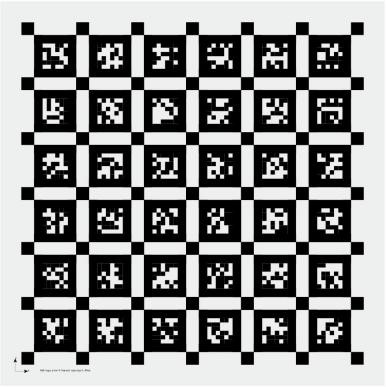
\includegraphics[width=0.5\textwidth]{figures/april_board}
    \caption{April Board上印制的二维码和棋盘格图案}
    \label{fig:april_board}
\end{figure}

本文中使用的标定物体为April Board,即印有二维码和棋盘格组成的图案的标定板,如图\ref{fig:april_board}所示。
该标定板的尺寸为$800 \times 800$毫米,每个二维码的边长为$88$毫米。
该图案中棋盘格的十字角点可由算法精确完成亚像素级定位,而密集的二维码则便于在不同相片中便捷地匹配角点。
其采用了玻璃基板,以保证标定板的刚性和平整度;
同时采用了氧化铝表面,使标定板表面无明显镜面反射光斑,确保标定板在不同光照条件下的可靠性。

在拍摄标定物体时,首先将相机固定到支架上,将任意物体摆放至预计人脸的位置作为调节的参照,并完成相机角度调节和对焦操作。
将相机切换至手动对焦模式,关闭光学防抖,以防止其内外参意外发生变化。
然后,撤走参照物,将标定板放在该位置,使用前述(第\ref{sec:passive_sync}节)被动相机同步装置同时触发所有相机进行拍摄。转动标定板,重复触发15-20次快门。

\paragraph{相机标定原理}本文中的相机标定算法接收照片中的特征点坐标作为输入,求解上述相机模型中的参数$\delta$。
正式地,假设共触发了$M$次快门,标定板中共有$K=144$个角点,算法的输入包括第$i$个相机的第$j$次触发快门拍摄中的第$k$个角点($j = 1,2,\cdots,M$、$k = 1,2,\cdots,K$)在像素坐标系中的坐标$o_{i,j,k}\in \mathbb{R}^2$;
以及角点在标定板坐标系中的坐标$w_k\in \mathbb{R}^3$。
由于每次触发快门时标定板都由人工转动,因此其在世界坐标系中的位置也是未知的,故将第$j$次快门时标定板坐标系到世界坐标系的刚体变换$T_{j}(\cdot)\in SE(3)$也做为未知量。
其中固定$T_{1}$为幺元,即$T_{1}(X) = X$,以确定世界坐标系的位置。
则本文中的相机标定问题可以表示为以下最小二乘优化问题:
\begin{equation}
    \label{eq:calib_opt}
    \argmin_{\delta,T} \sum_{i,j,k} \left\| o_{i,j,k} - \pi\left(\delta_i, T_j(w_k)\right) \right\|^2
\end{equation}

本节剩余部分将介绍角点的识别、精确定位,模型初始化及上述优化问题的具体求解方法。

\paragraph{二维码、角点识别}为识别标定板中可供拟合的角点,本文首先识别照片中的二维码,并将二维码的四个角作为角点的候选点。
本文所用标定板上的二维码为AprilTag,本文实现的识别算法也是基于其开源的方法\cite{AprilTag}。
该算法是一个自下而上的算法,它首先从照片中识别直线段,然后将直线段组合成四边形,最后试图将四边形区域识别为二维码。得益于二维码的纠错功能,虽然该方法召回率稍低,但查准率非常高。同时二维码中存储的信息可用于角点在不同照片中的匹配。

本文所实现的版本的输入为相机拍摄的,原始Bayer格式的照片,其中RGB像素排列,如图\ref{fig:bayer}所示,每$2\times 2$个像素中包括一个红色像素、两个绿色像素和一个蓝色像素。
将原始照片记为$I\in \mathbb{R}^{H\times W}$,其中$H$和$W$分别为照片的高和宽。
其中,红色像素记为$I^R\in \mathbb{R}^{\frac{H}{2}\times \frac{W}{2}}$,绿色和蓝色像素同理记为$I^G$和$I^B$。进一步,位于红色像素右边的像素记为$I^{G1}$,位于红色像素下方的记为$I^{G2}$。
通常数码相机进行的降噪、锐化等处理对标定并无帮助,因此本文直接使用原始照片。

\begin{figure}
    \centering
    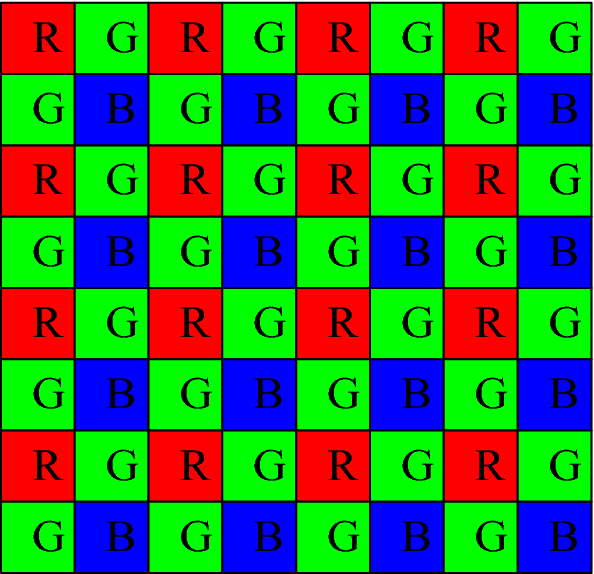
\includegraphics[width=0.4\textwidth]{figures/bayer}
    \caption{Bayer格式照片示意图}
    \label{fig:bayer}
\end{figure}

由于我们所拍摄的照片分辨率远超二维码识别所需,因此本文先对照片进行降采样。
其具体方法是,首先只取$I^{G1}$,以排除颜色对二维码识别的影响。
再对$I^{G1}$进行5倍平均池化,即降采样后的照片$I_{\text{down}}$的尺寸为$\frac{H}{10}\times \frac{W}{10}$。以此降低算法耗时并大大降低照片中的噪声等级,提升算法的鲁棒性。
在的分辨率的图像上完成二维码识别后,二维码的四个角的坐标$o^\mathrm{down}$将被重新映射回完整分辨率的像素坐标,以初始化后续的精确定位步骤:
\begin{equation}
    \tilde{o} = 10 \cdot o^\mathrm{down} + [5,4]
    \text{,}
\end{equation}
注意此处每个像素坐标系的原点均定义在左上角的像素的中心点,因此需要加入额外的偏移量,以确保所得到的$\tilde{o}$是$o$的无偏估计。

% 本文使用的相机拍摄的原始照片分辨率高,可达$5472\times 3648$;
% 且宽容度高,其量化后的亮度可达约13000级,相比普通JPG照片仅有256级。
% 因此,本文在\cite{AprilTag}的基础上,设计了尺度、亮度无关的直线段识别算法,使其更加鲁棒,并减少算法超参数调节的麻烦。
% \TODO{尺度、亮度无关的直线段识别算法}

\paragraph{角点精确定位}在上一步识别出角点后,依据角点周围的像素值,获取这些角点尽可能精确的像素坐标$o_{i,j,k}$,以保证标定的精度。
该步骤的难点在于,算法需要对失焦造成的模糊、成像过程中的噪声等因素足够鲁棒,并达到亚像素级的精度。

本文采用的算法为\citet{ROCHADE}提出的精确角点定位算法,其基本思想为:
使用一个二维多项式函数对角点周围的像素进行拟合,然后以该多项式函数的鞍点作为该角点的精确像素坐标。

具体地,本文首先需要从照片原始数据获取单通道灰度图。
为此,需要拟合R、B两个通道和G通道的比例系数(也即求白平衡系数),这两个系数与环境光照、标定板材质等有关。
本文假设标定板任意位置的饱和度为0,即RGB三通道的像素值应相等。
为求系数,本文首先对上一步求得的二维码区域求凸包,以定位照片中的标定板。
记照片原始数据为$I$,凸包区域为$A$,则所求灰度图$\bar{I}$为:
\begin{equation}
    \label{eq:wb}
    \begin{cases}
        \bar{I}^G = I^G \\
        \bar{I}^R = I^R \frac{\sum_{i\in A}{I^{G1}_i + I^{G2}_i}}{\sum_{i\in A}{I^R_i}} \\
        \bar{I}^B = I^B \frac{\sum_{i\in A}{I^{G1}_i + I^{G2}_i}}{\sum_{i\in A}{I^B_i}}
    \end{cases}\text{。}
\end{equation}
然后,对该图使用半径为$r$的圆锥形kernel进行滤波,以使像素值平滑,从而能更好地被多项式函数拟合。
最后,以角点的当前估计位置为中心,使用二阶二维多项式函数对周围的$2r+1 \times 2r+1$个像素进行最小二乘拟合:
\begin{equation}
    \label{eq:poly}
    \hat{a} = \argmin_{a} \sum_{x,y} \left(\bar{I}(x, y) - (a_0 x^2 + a_1 y^2 + a_2 xy + a_3 x + a_4 y + a_5)\right)^2\text{。}
\end{equation}
在实现上,本文直接使用解析公式求解该线性最小二乘问题。最后,求该二维多项式函数的鞍点作为该角点新的估计位置:
\begin{equation*}
    \Delta = 4 \hat{a}_0 \hat{a}_1 - \hat{a}_2^2
\end{equation*}
\begin{equation}
    \label{eq:subpixel}
    \begin{cases}
        x' = -\frac{\hat{a}_2 \hat{a}_4 - 2 \hat{a}_1 \hat{a}_3}{\Delta} \\
        y' = -\frac{\hat{a}_2 \hat{a}_3 - 2 \hat{a}_0 \hat{a}_4}{\Delta}
    \end{cases}\text{,}
\end{equation}
并如此迭代,直到角点的估计位置收敛,该收敛的位置即为$o$。
在此过程中,若估计位置超出了图像范围,或$\Delta < 0$,则将该角点排除。
$\Delta < 0$的原因通常是该角点被其他物体遮挡,或者受到其他物体投下的阴影影响。

在该算法中,$r$的选取可能对结果产生较大影响。较大的$r$将能利用照片中更多像素的信息,从而对噪声更加鲁棒,但也不能过大,否则周边的二维码,或相邻的其他角点等无关信息将影响拟合结果。为此,本文依据上一步识别到的二维码的尺寸以自适应地选择$r$。令$\hat{o}_{i,j}$为照片中第$i$个二维码的第$j$个角点的估计位置,$j\in\{1,2,3,4\}$,以顺时针方向排列,则$r$的选取为:
\begin{equation}
    \label{eq:r}
    \begin{aligned}
        l_{i,\textrm{edge}} & = \min_j\left(\|o_{i,j} - o_{i,j+1\mod 4}\|\right)\text{,} \\
        l_{i,\textrm{diag}} & = \min\left(\|o_{i,1} - o_{i,3}\|, \|o_{i,2} - o_{i,4}\|\right)\text{,} \\
        r & = \min_i\left\{0.07 l_{i,\textrm{edge}}, 0.05 l_{i,\textrm{diag}}\right\}\text{。}
    \end{aligned}
\end{equation}

\paragraph{多相机内参标定与外参传递}
在第一阶段,本文将对每台相机分别进行标定,获得各相机的内参初始化值
并估计标定版在每次触发快门时与各台相机的相对位置。
具体地,本文依据相机和镜头厂商提供的传感器尺寸、图像分辨率、镜头焦距初始化相机内参$f$、$c$,使用PnP算法求解标定板在每次触发快门时与相机的相对位置$T_{i,j}$;
然后使用Levenberg-Marquardt算法对这些参数进行调整。

由于不同相机的同一次快门的触发是严格同步的,因此可以认为若不同相机在同一次快门的触发时,拍摄到的标定板在世界坐标系中的位置是相同的。
据此可将每台相机,以及每次快门触发作为节点,构建二部图,图中的边表示该相机在该次快门中拍摄到了标定板。
若该二部图是连通图,则可迭代地将所有相机、所有快门触发中的标定板的位置传递到世界坐标系中,
如算法\ref{alg:calib_init}所示。
并最终获得$\delta$和$T$中所有参数的初始化值。

\begin{algorithm}[t]
    \caption{外参传递}
    \label{alg:calib_init}
    \begin{algorithmic}[1]
        \Require 连通二部图$(V,E)$;第$j$次快门时标定版坐标系到相机$i$坐标系的刚体变换$\hat{T}_{i,j}\in SE(3),(i,j)\in E$
        \Procedure{外参传递}{$V,E,\hat{T}_{i,j}$}
            \State $C \gets \emptyset$\Comment{已传递的相机集合}
            \State $T_{1} \gets \mathbf{I}$\Comment{以第$1$次快门时标定版坐标系作为世界坐标系}
            \State $S \gets \{1\}$\Comment{已传递的快门触发集合}

            \While{$C \cup S \neq V$}
                \State $i \gets \forall i\in V| i\notin C, \exists j\in S| (i,j)\in E$
                    \Comment{选择与已知位置的标定板相邻的相机}
                \State $U_{i} \gets T_{j}\hat{T}_{i,j}^{-1}$
                    \Comment{相机$i$到世界坐标系的变换}
                \State $C \gets C \cup \{i\}$
                \ForAll{$j | (i,j)\in E, j\notin S$}
                    \State $T_{j} \gets U_{i}\hat{T}_{i,j}$
                        \Comment{第$j$次快门时标定版到世界坐标系的变换}
                \EndFor
                \State $S \gets S \cup \{j\in V| (i,j)\in E\}$
            \EndWhile
            \State \Return $U, T$
        \EndProcedure
    \end{algorithmic}
\end{algorithm}

\paragraph{集束调整}在第二阶段,本文将对所有相机进行集束调整,即直接使用公式\eqref{eq:calib_opt}中的目标函数,在上一阶段的初始化值的基础上,对模型中的所有参数进行优化。
具体地,本文使用了Levenberg-Marquardt算法\cite{lm},对目标函数进行优化求解。
并手动实现了公式\eqref{eq:calib_opt}的雅克比矩阵的解析求解算法,以提升算法的速度和收敛精度。

然后,排除掉误差较大的角点,再次重复上述优化过程,并如此迭代数次,每次使用更严格的误差阈值进行排除。
这些误差较大的角点通常是由于角点定位不准确造成的,因此,将其排除后可以提高标定的精度。

\paragraph{标定结果和误差分析}

由于本文采用的模型参数量小,且角点数量多(约15000个),基本没有过拟合的风险。
因此本文并未单独划分验证集,而是直接使用所有的角点的重投影误差作为标定精度的评价标准。
平均重投影误差定义为:
\begin{equation}
    \label{eq:reproj_err}
    \text{reproj\_err} = \frac{1}{\|O\|}\sum_{(i,j,k)\in O}\left\|o_{i,j,k} - \pi\left(\delta_i, T_j(w_k)\right)\right\|_2
    \text{,}
\end{equation}
其中,$O$为所有可用角点集合。注意该指标与公式\eqref{eq:calib_opt}中的目标函数有所不同,该指标是所有角点的重投影误差的算术平均,以便于进行下文中的各种统计。
上述方法最终获得的平均重投影误差为0.38像素。
以下将对可能影响标定精度的各个因素进行分析:

\begin{enumerate}
\item 自动对焦:由于现实中的相机不是理想的针孔相机,仅有处于焦平面上的物体能清晰成像。
为获得清晰的照片,相机通常默认会开启自动对焦。即通过电机驱动镜片移动,以改变焦平面的距离。
但不幸的是,镜片的移动同样也会导致相机的成像参数发生较大变化,从而无法达到较高的标定精度。
在实践中,若开启了自动对焦,我们则无法获得优于5像素的重投影误差。
因此,在标定和采集数据时设置手动对焦是非常必要的。

\begin{figure}
    \centering
    \import{build/figures}{stab_ablation.pgf}
    \caption[不同相机的重投影误差]{同一次标定中不同相机第一阶段的重投影误差。其中,10号相机开启了光学防抖,其余相机关闭了光学防抖。}
    \label{fig:stablize_ablation}
\end{figure}

\item 光学防抖:为尽量避免相机机身震动引起的运动模糊,本文使用的镜头配备有光学防抖功能。该功能的原理也是通过电机驱动镜片运动以抵消相机机身的运动的影响。
但是即使本文中的相机是固定在支架上的,光学防抖功能仍然会导致外参的轻微变化。
如图\ref{fig:stablize_ablation}所示,图中仅10号相机开启了防抖,而其重投影误差超出了其他相机近一倍。
因此,关闭光学防抖将有助于提高标定精度。但需注意,关闭防抖后,每次物理接触相机调节参数等之后,再次拍摄前均需要等待5-10秒,以允许整个支架系统恢复稳定。

\begin{table}[htb]
    \centering
    \begin{tabular}{l|S[table-format=2.3] S[table-format=1.3]}
        \toprule
        畸变模型(参数数量) & \shortstack{集束调整前\\重投影误差(像素)} & 重投影误差(像素) \\
        \midrule
        无畸变 (0) & 20.22 & 7.01 \\
        默认 (5) & 0.917 & \textbf{0.455} \\
        rational (8) & 0.762 & 0.462 \\
        thin prism (12) & 1.314 & 0.445 \\
        tilted (14) & 0.744 & 0.449 \\
        \bottomrule
    \end{tabular}
    \caption[相机畸变模型对标定精度的影响]{OpenCV中实现的各种相机畸变模型对标定精度的影响。加粗数字为本文最终使用模型。}
    \label{tab:distortion}
\end{table}

\item 相机畸变模型:相机镜头会带来少量畸变,从而使成像结果与理想的针孔相机成像结果有所差异。
本文使用了OpenCV中默认的具有5个参数的畸变模型,以建模这种差异。
图\ref{tab:distortion}展示了使用不同畸变模型时重投影误差。
可见本文所使用的相机具有不可忽视的镜头畸变,对畸变进行建模可大幅提高标定精度。
另一方面,使用更为复杂的畸变模型则没有明显的优势。

\begin{figure}
    \centering
    \import{build/figures}{corner_fit.pgf}
    \small
    (a) 不同标定板角度下的精度对比\hfill
    (b) 不同失焦模糊下的精度对比\hfill
    (c) 不同噪音下的精度对比
    \caption[OpenCV与本文使用的角点定位算法的精度对比]{
        OpenCV与本文使用的角点定位算法的精度对比。
        带有噪音的图像服从柏松分布,
        增益表示在传感器取得最大读数时接收的电子数量,增益越高,噪声越小。
        在Blender渲染的全部1000张图像中,
        (a)展示了增益$2^{14}$时距离焦平面-0.3至0.2米的图像中,误差与标定版角度的关系;
        (b)展示了增益$2^{14}$时倾斜角度70°以下的图像中,误差与失焦模糊程度的关系;
        (c)展示了距离焦平面-0.3至0.2米且倾斜角度70°以下的图像中,误差与噪音强度的关系。
    }
    \label{fig:corner_fit}
\end{figure}

\begin{figure}
    \centering
    \begin{subfigure}{1.57in}
        \import{build/figures}{corner_gain-14_0023_opencv.pgf}%
        \caption{OpenCV, 增益$2^{14}$}%
    \end{subfigure}%
    \begin{subfigure}{1.57in}
        \import{build/figures}{corner_gain-10_0023_opencv.pgf}%
        \caption{OpenCV, 增益$2^{10}$}%
    \end{subfigure}%
    \begin{subfigure}{1.57in}
        \import{build/figures}{corner_gain-14_0023_saddle.pgf}%
        \caption{本文, 增益$2^{14}$}%
    \end{subfigure}%
    \begin{subfigure}{1.57in}
        \import{build/figures}{corner_gain-10_0023_saddle.pgf}%
        \caption{本文, 增益$2^{10}$}%
    \end{subfigure}%
    \caption[较严重失焦时的角点定位结果]{
        较严重失焦时的角点定位结果。
        左边两幅图展示了OpenCV的cornerSubPix算法在不同噪音强度时的结果,
        右边两幅图展示了本文所实现的算法的结果。
        可见OpenCV无法正确收敛,在同等半径参数下,本文所实现的算法可处理更大的失焦程度。
    }
    \label{fig:corner_blur}
\end{figure}

\item 角点定位算法:角点定位的精度是决定标定精度的关键因素。
为验证本文所实现的算法的性能,本文使用Blender的Cycles渲染器生成了1000张的标定板角点的图像,
这些角点具有随机的位置、角度、失焦模糊和噪声,
并在这组图像上将本文所实现的算法和OpenCV的cornerSubPix算法进行了对比。
具体方法是使用同样的半径$r=15$,使用不同算法分别在每张图像的角点真值附近$10\times 10$像素的范围内随机初始化100次,并优化到收敛,然后统计每张图像的平均重投影误差。
如图\ref{fig:corner_fit}所示,本文在整体精度上大幅优于OpenCV的算法,且在应对极端角度,失焦模糊,随机噪声这些采集中经常出现的情况也有较高的鲁棒性。
而OpenCV的算法在较严重的失焦时则无法正确收敛(如图\ref{fig:corner_blur})。

\item 角点定位失败造成的外点:由于角点被其他物体遮挡,或者受到其他物体投下的阴影影响,偶尔角点定位会收敛到错误的位置,造成外点。
但这样的点很少,通常小于10个,因此在实践中未观察到对标定精度有显著的影响。
但是,在统计损失函数或平均重投影误差时,排除这些点可使所得统计数据更能代表整体标定精度。

\begin{table}[htb]
    \centering
    \begin{tabular}{l|rrr}
        \toprule
        图像源 & 定位成功角点数 & 离群点 & 重投影误差(像素) \\
        \midrule
        原始图像(本文)  & 14730 & 8 & 0.3753 \\
        Canon DDP后处理 &  &  & \\
        相机JPG预览图    & 14589 & 11 & 0.3588 \\
        \bottomrule
    \end{tabular}
    \caption{不同后处理方案对标定精度的影响}
    \label{tab:camera_postprocess}
\end{table}

\item 相机后处理:数码相机为呈现更加视觉友好的图像,会对采集的数据进行一系列后处理,如去马赛克,gamma映射、降噪、锐化、白平衡等。
为验证这些功能对标定精度可能的影响,本文对比了使用处理前和处理后的数据标定的重投影误差,如表\ref{tab:camera_postprocess}所示。
其中后处理使用的是佳能Digital Photo Professional软件,并在默认设置的基础上开启了数码镜头校正,未开启镜头畸变校正。它处理一张图片需要约30秒的时间,对于12台相机共数百张图片来说需要耗费的时间相当可观。
\TODO{实验显示两者并无显著区别,简单起见,本文选择了直接使用用原始数据。}
\end{enumerate}
